
\documentclass[aspectratio=169,14pt,xcolor=dvipsnames]{beamer}
\usepackage[utf8]{inputenc}
\usepackage{enumerate}
\usepackage[ngerman]{babel}
\usepackage[T1]{fontenc}
\usepackage{lmodern}
\usepackage{blindtext}
\usepackage{pdfpages}
\usepackage[font=footnotesize]{caption}
\usepackage{fancyhdr}
\usepackage{extramarks}
\usepackage[]{hyperref}
\usepackage{array}
\usepackage{longtable}
\usepackage{xcolor}
\usepackage{colortbl}
\usepackage{graphicx}
\usepackage{amssymb}
\usepackage{eurosym}
\usepackage{pgfpages}
\usepackage{xfrac}
\usepackage{here}
\usepackage{listings}
\usepackage{makecell}
\usepackage{tikz}
\usepackage[yyyymmdd,hhmmss]{datetime}
% we want ER + above/below + left/right
\usetikzlibrary{er,positioning}
%\usepackage{csvsimple}
\usetheme[width=0.17\textwidth]{Hannover}
\usecolortheme{owl}
\usefonttheme{professionalfonts}

\definecolor{lightgray}{rgb}{0.7,0.7,0.7}
\definecolor{gray}{rgb}{0.5,0.5,0.5}
\definecolor{darkgray}{rgb}{0.3,0.3,0.3}

\setbeamertemplate{caption}[numbered]
\setbeamerfont{title}{size=\normalsize}
\setbeamercolor{frametitle}{fg=gray}
\setbeamercolor{framesubtitle}{fg=lightgray}

\definecolor{cyan}{HTML}{7FFFD4}
\definecolor{purple}{rgb}{0.65, 0.12, 0.82}

\lstdefinelanguage{JavaScript}{
  keywords={typeof, new, true, false, catch, function, return, null, catch, switch, var, if, in, while, do, else, case, break},
  keywordstyle=\color{Cerulean}\bfseries,
  ndkeywords={class, export, boolean, throw, implements, import, this, extends, state, props},
  ndkeywordstyle=\color{cyan}\bfseries,
  identifierstyle=\color{lightgray},
  sensitive=false,
  comment=[l]{//},
  morecomment=[s]{/*}{*/},
  commentstyle=\color{purple}\ttfamily,
  stringstyle=\color{red}\ttfamily,
  morestring=[b]',
  morestring=[b]"
}
%definitionen für Code snippet, einbinden mit  \lstinputlisting{unitetest.js}
\lstdefinestyle{mystyle}{
    language=JavaScript,
    backgroundcolor=\color{darkgray},
    numberstyle=\tiny\color{gray},
    basicstyle=\ttfamily\footnotesize,
    breakatwhitespace=false,
    breaklines=true,
    captionpos=b,
    keepspaces=true,
    numbers=left,
    numbersep=5pt,
    showspaces=false,
    showstringspaces=false,
    showtabs=false,
    tabsize=2
    }
\lstset{style=mystyle}

\newcommand{\datum}{22.01.2021} %Datum des Vortrags

\title{Frameworks}
\author[]{Laura Pech}
\institute{Unitedprint.com SE\\Auszubildende Fachinformatikerin für Anwendungsentwicklung}
\date{\datum}

\addtobeamertemplate{navigation symbols}{}{%
\usebeamerfont{button}%
\usebeamercolor{black}%
\hspace{3em}%
\huge{\insertframenumber/\inserttotalframenumber}
}

\setbeamertemplate{footline}[text line]{%
\parbox{\linewidth}{\vspace*{-8pt}\datum\hfill\insertauthor\hfill\insertframenumber/\inserttotalframenumber}}
\setbeamertemplate{navigation symbols}{}

\setcounter{tocdepth}{1}

\begin{document}
\maketitle

\begin{frame}[t]
    \frametitle{Gliederung}
    \hypersetup{linkcolor=black}
    \tableofcontents%[subsubsectionstyle=hide]
\end{frame}

\section{Was ist ein Framework?}
\begin{frame}[t]
    \frametitle{\secname}
    \begin{itemize}
        \setlength{\itemsep}{1.5em}
        \item Rahmenstruktur oder Programmiergerüst
        \item bietet Werkzeuge für coding
        \item Codebausteine
        \item auf den Anwendungsfall beschränkt
    \end{itemize}

\end{frame}

\begin{frame}[t]
    \frametitle{\secname}
    \begin{itemize}
        \setlength{\itemsep}{1.5em}
        \item genormte Schnittstellen
        \item häufigster Nutzungsgrund sind Klassenbibliotheken
        \item Verwendung mehrerer Frameworks möglich
    \end{itemize}
\end{frame}

\section{Aufbau von Frameworks}
\subsection{Laufzeitumgebung}
\begin{frame}[t]
    \frametitle{\subsecname}
    \framesubtitle{\secname}
    \begin{itemize}
        \setlength{\itemsep}{1.5em}
        \item "Runtime system"
        \item Konfiguration aus Hardware und Software
        \item Fürht Code aus
    \end{itemize}
\end{frame}

\subsection{Virtuele Maschiene}
\begin{frame}[t]
    \frametitle{\subsecname}
    \framesubtitle{\secname}
    \begin{itemize}
        \setlength{\itemsep}{1.5em}
        \item optional, nicht bei allen Frameworks
        \item zur Überprüfung von Applicationen auf Funktionalität
        \item Beispiel JRE mit der Java Virtual Machiene
    \end{itemize}
\end{frame}

\subsection{Elemente}
\begin{frame}[t]
    \frametitle{\subsecname}
    \framesubtitle{\secname}
    Libraries
    \begin{itemize}
        \setlength{\itemsep}{1.5em}
        \item "Klassenbibliotheken"
        \item Framework != Library
    \end{itemize}
\end{frame}

\begin{frame}[t]
    \frametitle{\subsecname}
    \framesubtitle{\secname}
    Klassen
    \begin{itemize}
        \setlength{\itemsep}{1.5em}
        \item strukturierte Sammlung von Methoden und Attributen
        \item Vordefiniert durch Framework
        \item müssen nur mit Daten gefüllt werden
    \end{itemize}
\end{frame}

\begin{frame}[t]
    \frametitle{\subsecname}
    \framesubtitle{\secname}
    API's
    \begin{itemize}
        \setlength{\itemsep}{1.5em}
        \item ''Application Programming Interfaces"
        \item vordefinierte Programmierschnittstellen
        \begin{itemize}
            \item z.B. zu Datenbanken oder MVC
        \end{itemize}
    \end{itemize}
\end{frame}

\section{Arten von Frameworks}
\subsection{Web Frameworks}
\begin{frame}[t]
    \frametitle{\subsecname}
    \framesubtitle{\secname}
    Backend Frameworks
    \begin{itemize}
        \setlength{\itemsep}{1.5em}
        \item regelt zum Beispiel:
        \begin{itemize}
            \setlength{\itemsep}{1.5em}
            \item Datenzugriffe
            \item schützt interne Bereiche
            \item Reglung von Benuter Logins
            \item wichtige Hintergrundaufgaben z.B. Effizienz oder Server-Client Kommunikation
        \end{itemize}
    \end{itemize}
\end{frame}

\begin{frame}[t]
    \frametitle{\subsecname}
    \framesubtitle{\secname}
    Frontend Frameworks
    \begin{itemize}
        \setlength{\itemsep}{1.5em}
        \item regelt zum Beispiel
        \begin{itemize}
            \setlength{\itemsep}{1.5em}
            \item Gestaltung des Frontends -> responsive Webdesign
            \item Data-Binding -> Handling von Daten zwischen Objekten
        \end{itemize}
    \end{itemize}
\end{frame}

\subsection{App Frameworks}
\begin{frame}[t]
    \frametitle{\subsecname}
    \framesubtitle{\secname}
    \begin{itemize}
        \setlength{\itemsep}{1.5em}
        \item Native Apps
        \item Web Apps
        \item Hybride Apps
    \end{itemize}
\end{frame}

\subsection{Software Frameworks}
\begin{frame}[t]
    \frametitle{\subsecname}
    \framesubtitle{\secname}
    \begin{itemize}
        \setlength{\itemsep}{1.5em}
        \item zur Entwicklung von System- und Anwendungssoftware
        \item kann Schnittstellen zur Hardware bieten
        \item ist eigentlich Überbegriff für Frameworkarten
    \end{itemize}
\end{frame}

\subsection{Test Frameworks}
\begin{frame}[t]
    \frametitle{\subsecname}
    \framesubtitle{\secname}
    \begin{itemize}
        \setlength{\itemsep}{1.5em}
        \item Unit-Tests
        \item Nachweisen von Fehlern in Komponenten der Software
    \end{itemize}
\end{frame}

\section{Beispiele}
\subsection{Catalyst}
\begin{frame}[t]
    \frametitle{\subsecname}
    \framesubtitle{\secname}
    \begin{itemize}
        \setlength{\itemsep}{1.5em}
        \item Mariposa basiert darauf
        \item MVC Framework für Perl
        \item Session Handeling und Authorsierung
        \item Datenbankmanipulations Schnittstellen (nicht von uns genutzt)
    \end{itemize}
\end{frame}

\subsection{.NET}
\begin{frame}[t]
    \frametitle{\subsecname}
    \framesubtitle{\secname}
    \begin{itemize}
        \setlength{\itemsep}{1.5em}
        \item Objektorientiert
        \item Common Language Runtime (CLR) + Klassenbibliothek
        \item Anwendungsentwicklung für Microsoft
        \item erzwingt Typensicherheit
    \end{itemize}
\end{frame}

\begin{frame}[t]
    \frametitle{\subsecname}
    \framesubtitle{\secname}
    \begin{itemize}
        \setlength{\itemsep}{1.5em}
        \item Funktionen z.B. Dateizugriffe, Netzwerkkommunikation, Datenbankzugriffe, Grafik und grafische Benutzeroberflächen
        \item Methoden z.B. Hashfunktionen, Zeit- und Datumsberechnung sowie -konvertierung oder Funktionen aus der alltäglichen Mathematik
    \end{itemize}
\end{frame}

\subsection{Laravel}
\begin{frame}[t]
    \frametitle{\subsecname}
    \framesubtitle{\secname}
    \begin{itemize}
        \setlength{\itemsep}{1.5em}
        \item PHP Framework
        \item weitgefächert - komplettes System abbildbar
    \end{itemize}
\end{frame}

\begin{frame}[t]
    \frametitle{\subsecname}
    \framesubtitle{\secname}
    \begin{itemize}
        \setlength{\itemsep}{1.5em}
        \item Funktionen z.B.:
        \begin{itemize}
            \setlength{\itemsep}{1.5em}
            \item Routing
            \item Authentifikation und Authorisierung
            \item Datenbankschnittstellen zu verschiedensten Datenbanken
            \item Session Handling
        \end{itemize}
    \end{itemize}
\end{frame}

\subsection{Bootstrap}
\begin{frame}[t]
    \frametitle{\subsecname}
    \framesubtitle{\secname}
    \begin{itemize}
        \setlength{\itemsep}{1.5em}
        \item HTML und CSS basierende Gestaltungsvorlagen für z.B.
        \begin{itemize}
            \setlength{\itemsep}{1em}
            \item Typografie
            \item Formulare
            \item Tabellen
            \item Grid-Systeme
            \item Navigations- und andere Oberflächengestaltungselemente
        \end{itemize}
        \item optionale JavaScript-Erweiterungen
    \end{itemize}
\end{frame}

\section{ReactJs}
\subsection{Was ist das und warum wird es genutzt?}
\begin{frame}[t]
    \frametitle{\subsecname}
    \framesubtitle{\secname}
    \begin{itemize}
        \setlength{\itemsep}{1.5em}
        \item Rendering
        \item Wiederverwendbarkeit
        \item Umwandlung zu native App durch "React Native" möglich
    \end{itemize}
\end{frame}

\subsection{Konzepte}
\begin{frame}[t]
    \frametitle{\subsecname}
    \framesubtitle{\secname}
    Element rendering
    \lstinputlisting{js/rendering.js}
\end{frame}

\begin{frame}[t]
    \frametitle{\subsecname}
    \framesubtitle{\secname}
    Components und Props
    \lstinputlisting{js/components.js}
\end{frame}

\begin{frame}[t]
    \frametitle{\subsecname}
    \framesubtitle{\secname}
    State
    \lstinputlisting{js/state.js}
\end{frame}

\begin{frame}[t]
    \frametitle{\subsecname}
    \framesubtitle{\secname}
    Lifecycle
    \begin{figure}[t]
        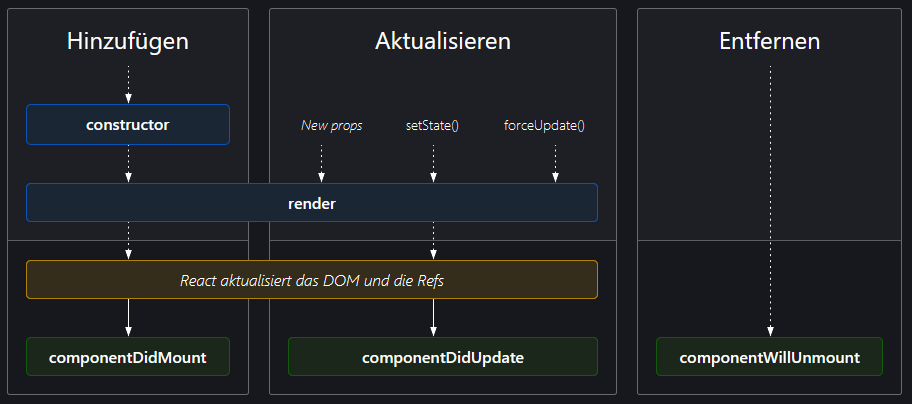
\includegraphics[width=0.8\textwidth]{images/React_lifecycle.png}
        \centering
        \caption{Lifecycle ReactJs}
    \end{figure}
\end{frame}

\begin{frame}[t]
    \frametitle{Quellen}
    \scriptsize https://www.tenmedia.de/de/glossar/entwicklungsframeworks, \newline letzter Aufruf \today\ \currenttime \newline \newline
    \scriptsize https://www.df.eu/blog/die-beliebtesten-backend-frameworks-fuer-ihren-webauftritt/, \newline letzter Aufruf \today\  \currenttime \newline \newline
    \scriptsize https://www.html-seminar.de/unterschied-seitenaufbau-fuer-mobiles-www.htm, \newline letzter Aufruf \today\  \currenttime \newline \newline
    \scriptsize https://de.wikipedia.org/wiki/.NET\_Framework, \newline letzter Aufruf \today\  \currenttime \newline \newline
    \scriptsize https://docs.microsoft.com/de-de/dotnet/framework/get-started/overview
    reactjs.org, \newline letzter Aufruf \today\ \currenttime \newline \newline
    \scriptsize https://de.wikipedia.org/wiki/Bootstrap\_(Framework), \newline letzter Aufruf \today\  \currenttime \newline \newline
    \scriptsize https://projects.wojtekmaj.pl/react-lifecycle-methods-diagram/, \newline letzter Aufruf \today\  \currenttime \newline \newline
\end{frame}

\end{document}